%
% Chapter 2 - Method
% ------------------
% Jul 1, 2015
%

\chapter{Developing optimal decadal records of Antarctic ice-shelf height change from multiple satellite radar altimeters}


\section*{}
\noindent
Antarctica's ice shelves, the floating extensions of the ice sheet, exert an important dynamic constraint on the flow of ice from the grounded ice sheet to the ocean, and hence on changes in global sea level. Thinning of an ice shelf reduces its ability to restrain the ice discharge from the grounded ice-sheet interior. However, our understanding of how ice-shelf processes couple ice-sheet changes to climate variability is still rudimentary. In part, this is due to the brevity and low resolution of surveys of ice-shelf thickness relative to the time scales on which ice-sheet mass fluctuates. We present optimal procedures to construct 18-year (1994--2012) time series of ice-shelf surface height around the entire Antarctic continent by merging data from multiple overlapping satellite radar altimeter missions (ERS-1, ERS-2, and Envisat). We apply an averaging scheme to enhance the signal-to-noise ratio of height changes over the floating ice shelves, and extract low-order polynomial trends using a robust approach accounting for both bias and variance in the fit (regularized regression with cross-validation). We identify the main processes affecting the estimation of ice-shelf height from satellite radar altimeters. We estimate uncertainties by bootstrap resampling of the residuals of the fit, allowing us to construct formal confidence intervals (unlike the standard error-propagation approach). Our results show that, for the ice shelves, densification of the surface is a more important effect than penetration of the radar signal in biasing the estimated height changes. The 18-year record of surface height allows us to map the temporal progression and spatial structure of changes in ice-shelf height, which provides insights on how ice shelves respond to the changing atmospheric and oceanic conditions.

\section{Introduction}

The Antarctic Ice Sheet contains ice above floatation equivalent to ~58 m of global sea-level rise \parencite{Fretwell2013} and, over centennial-to-millennial time scales, plays an important role in pacing sea-level changes \parencite{Alley2005}. Satellite measurements over the past two decades show mass loss from the grounded ice sheet \parencite{Shepherd2012} including accelerating loss in the Amundsen Sea Embayment \parencite{Sutterley2014}, a region with large potential for sea level rise contribution \parencite{Rignot2014, Joughin2014}. There is an urgent need to understand the mechanisms behind these current changes as a step towards predicting Antarctica's contribution to global sea-level change over the next century. 

Most ice mass loss from Antarctica takes place through iceberg calving and basal melting from the ice shelves, the floating extensions of the ice sheet \parencite{Depoorter2013, Joughin2012, Rignot2013}. Ice shelves restrain the discharge of grounded ice into the ocean through a buttressing effect \parencite{Joughin2011, Schoof2007}. Small perturbations in the adjacent oceanic and atmospheric conditions can have a large impact on the extent and thickness of ice shelves \parencite{Dutrieux2014, Rignot2004, Scambos2004}, which reduces their buttressing capability. The response of ice shelves to climate changes is, therefore, a key component in assessing future loss of grounded ice.

Our understanding of the many processes that affect ice-shelf mass balance is too rudimentary to allow prediction of ice-sheet change under projected future climate states. There are two complementary ways forward: to develop our theoretical framework of the actual mass-loss processes so they can be better represented in models; and to empirically relate observed ice-sheet change to ocean and atmospheric variability. In a recent study \parencite{Paolo2015} we reported changes in Antarctic ice shelf height, and inferred thickness during the 18-year period 1994--2012. The temporal and spatial resolutions of that record were ~3 months and ~30 km, respectively. This record will be used to improve knowledge of ice-shelf response to climate by comparing measured variability of ice thickness with measured or modeled changes in the ocean and atmosphere. This continuous, highly-resolved record overcomes the limitations of previous studies of ice-shelf thickness, which analyzed much shorter records and/or predominantly reported simple linear trends for large areas \parencite{Pritchard2012, Shepherd2010, Zwally2005}.

In this paper we document comprehensive methods for constructing continuous records from multiple satellite radar altimeters to obtain reliable time series of height change over the longest possible time period, providing detailed justification for the data processing approach used by \textcite{Paolo2015}. We present optimal procedures for merging data from three overlapping satellite missions, enhancing the signal-to-noise ratio of changes in ice-shelf height, and extracting 18-year mean trends and acceleration. We introduce an alternative approach to the standard error propagation for the uncertainty analysis: bootstrapping applied to time-dependent data. The method reveals complex patterns of ice-shelf height variability in both time and space.

\section{Satellite radar altimeter missions}
\label{sat-ra}

We used data from three European Space Agency (ESA) satellite radar altimeter (RA) missions: the European Remote Sensing Satellite-1 and Satellite-2 (ERS-1, 1991--1996; and ERS-2, 1995--2003); and the Environmental Satellite (Envisat, 2002--2012). Each satellite carried a standard pulse-limited altimeter with a footprint size of $\sim$3--5 km over the ice sheets. For reasons explained in Section \ref{sat-ra}, below, we do not use the first two years of ERS-1 data, resulting in an 18-year continuous record for 1994--2012.

ERS-1 was launched on July 1991 and operated between December 1991 and June 1996. It flew at an altitude of $\sim$785 km with an inclination of 98.5 degrees (latitudinal limit of 81.5$^\circ$), with three different orbital repeat periods: 3-day (Ice Phase, December 1991 to March 1992 and December 1993 to April 1993), 35-day (Multidisciplinary Phase, April 1992 to December 1993 and March 1995 to June 1996) and 168-day (Geodetic Phase, April 1994 to March 1995). ERS-2 was launched on April 1995 and operated from May 1995 to June 2003 in an orbit with a repeat period of 35 days, exactly following the ERS-1 35-day orbit. In June 2003 the on-board tape recorder used for the RA data failed, and the mission continued without altimetry until July 2011. The RA system on these two satellites was based on a linearly polarized antenna at 13.8 GHz Ku-band, yielding along-track measurements (several radar echoes averaged) that are $\sim$340 m apart (sampling rate of 20 Hz).

The ERS-1/ERS-2 orbit covered about 85\% of the Antarctic ice-shelf area, missing only the southern portions of the large Filchner-Ronne (Figure \ref{c2f1}) and Ross ice shelves. Over the ice shelves, ERS-1 and ERS-2 operated in both a standard 'ocean mode' and a specialized 'ice mode', alternating between them. The range window (the segment of return echo that is recorded) for ice mode was four times wider than for ocean mode, increasing the chances of capturing return signals over rough topographic surfaces. However the broader range window resulted in four times coarser sampling of the return waveform, leading to a less precise estimation of arrival time and, therefore, of the surface height.

Envisat was launched in March 2002 into the same 35-day orbit as ERS-1 and ERS-2, providing data at the same 20 Hz sampling rate. The altimeter on this satellite (RA-2) \parencite{Roca2009}, a linearly-polarized radar, operated via a single antenna dish on the Ku-band (13.6 GHz) and S-band (3.2 GHz). This dual frequency enables the correction of height-measurement errors introduced by the ionosphere. RA-2 had an improved precision over ice surfaces compared to the ERS altimeters, and operated with three sampling modes: 'fine', 'medium' and 'coarse', which differ by their sampling of the return waveform. Envisat stopped operating in April 2012.

We obtained Level-2 RA data as Ice Data Records (IDR) for each mission from the NASA/GSFC's Ice Altimetry group ({\tt http://icesat4.gsfc.nasa.gov/}). At GSFC, the RA waveforms were retracked using a multi-parameter range-retracking algorithm (the $\beta$-retracker) \parencite{Martin1983}. The following corrections were applied by GSFC: atmospheric range corrections; instrument corrections; slope corrections; ocean and solid earth tides \parencite{Brenner1983, Zwally2001, Zwally2005}; (for ERS) removal of a 40.9 cm bias from ERS-1 heights to account for a change in instrument parameter used for ERS-2 \parencite{Femenias1996}; corrections for drifts in the ultra-stable oscillator and bias changes in the scanning point target response that are obtained from ESA; and upgraded orbits (DGM-E04 orbits for ERS) which have a radial orbit precision of 5-6 cm \parencite{Scharroo1998}.


\begin{figure}[!ht]
  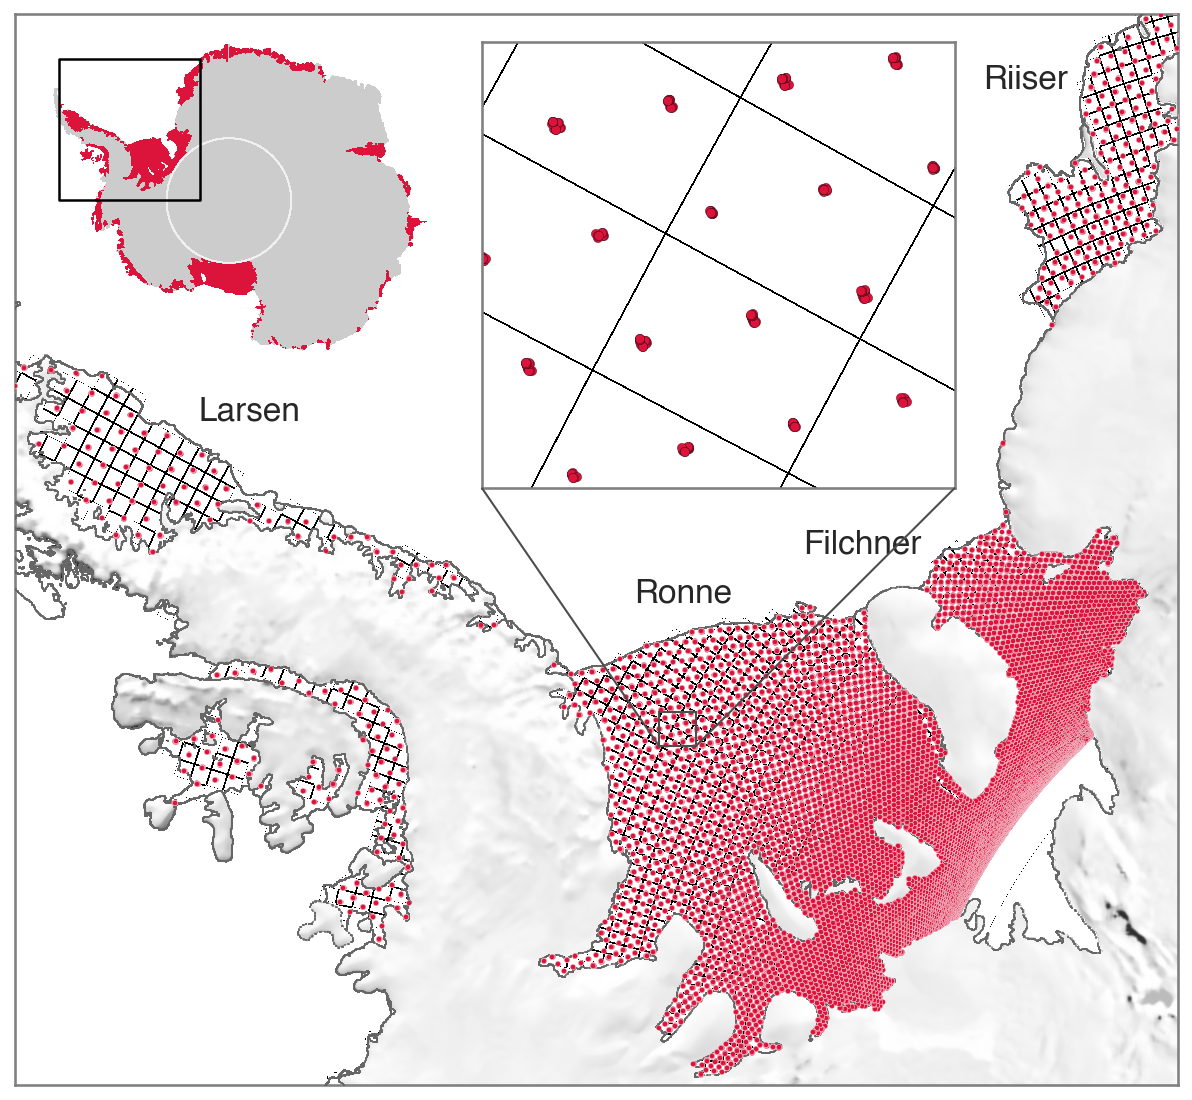
\includegraphics[width=\textwidth]{../img/map_xovers_grid_v8.png}
  \caption{ERS-1 radar altimeter data coverage over the Weddell Sea region of Antarctica for a typical 3-month period with the 35-day repeat orbit. Red dots are crossover locations on the ice shelves. The $\sim$30-km grid that we used to average the crossovers is overlaid. 
  ice shelves.} 
  \label{c2f1}
\end{figure}


\section{Processing satellite radar altimeter data}

Our determination of height changes over the ice shelves from multi-mission satellite RA data is based on crossover analysis [E.G.,]\parencite[e.g.,][]{Davis2004, Wingham2009, Zwally2005}, which estimates change in surface height at intersections between time-separated ascending and descending satellite tracks. Along-track analysis methods that provide higher point density have recently been introduced \parencite{Flament2012, Moholdt2010, Pritchard2012}; however, crossover analysis remains the most precise technique since differences are derived from precisely co-located height estimates on the ascending and descending tracks. The spacing of crossovers becomes much smaller as latitude approaches the satellite's turning point (Figure \ref{c2f1}).

In this section we describe the steps required to process RA data from multiple satellite missions. Steps include (see flowchart in Figure \ref{c2f2}): subsetting data over floating ice; data editing and additional corrections required for floating ice and for radar signal interactions with the surface layer on the ice shelves; crossover analysis; methods for merging data records from the different missions; and averaging scheme required to achieve satisfactory data coverage and accuracy. The output is 18-year long records of ice-shelf surface height, which we then analyzed using statistical techniques to derive long-term trends, acceleration and uncertainties.

\subsection{Initial RA data selection and editing}
\label{ra-processing}

\subsubsection{Antarctic ice shelf mask}

For this study we are interested only in Antarctica's floating ice shelves, and so we subsetted all of our RA datasets based on a 1-km resolution Antarctic ice-sheet mask \parencite{Depoorter2013} that was constructed using a composite of InSAR \parencite{Rignot2011}, ICESat \parencite{Brunt2010, Fricker2009}, MODIS MOA \parencite{Scambos2007} and ASAID \parencite{Bindschadler2011} products. This high-resolution product allows us to exclude all grounded ice, which includes islands, ice rises and rumples that are completely surrounded by ice shelves.

We considered only the portions of ice shelves that were present and afloat through the entire 18-year observation period. We excluded regions where ice front advance or retreat occurred during the 18 years and portions of a few ice shelves that ungrounded between 1994 and 2012.

\subsubsection{Altimeter data editing}

We excluded data if the following conditions were met: the return waveform had no leading edge, or had specular shape indicating surface melt ponds and melt streams \parencite{Phillips1998}; any geophysical correction was missing from the IDR; the crossover point was less than 3 km from any ice-shelf boundary (grounding line and ice front). The last criterion was designed to avoid biasing estimates (i) with high topographic gradients within the pulse-limited radar footprint, (ii) with changes in grounded ice that are an order of magnitude higher than over floating ice, and (iii) where geophysical corrections for ocean processes such tides are unreliable, especially close to the grounding line where the ice is not in full hydrostatic equilibrium \parencite{Fricker2006}.


\begin{figure}[!ht]
  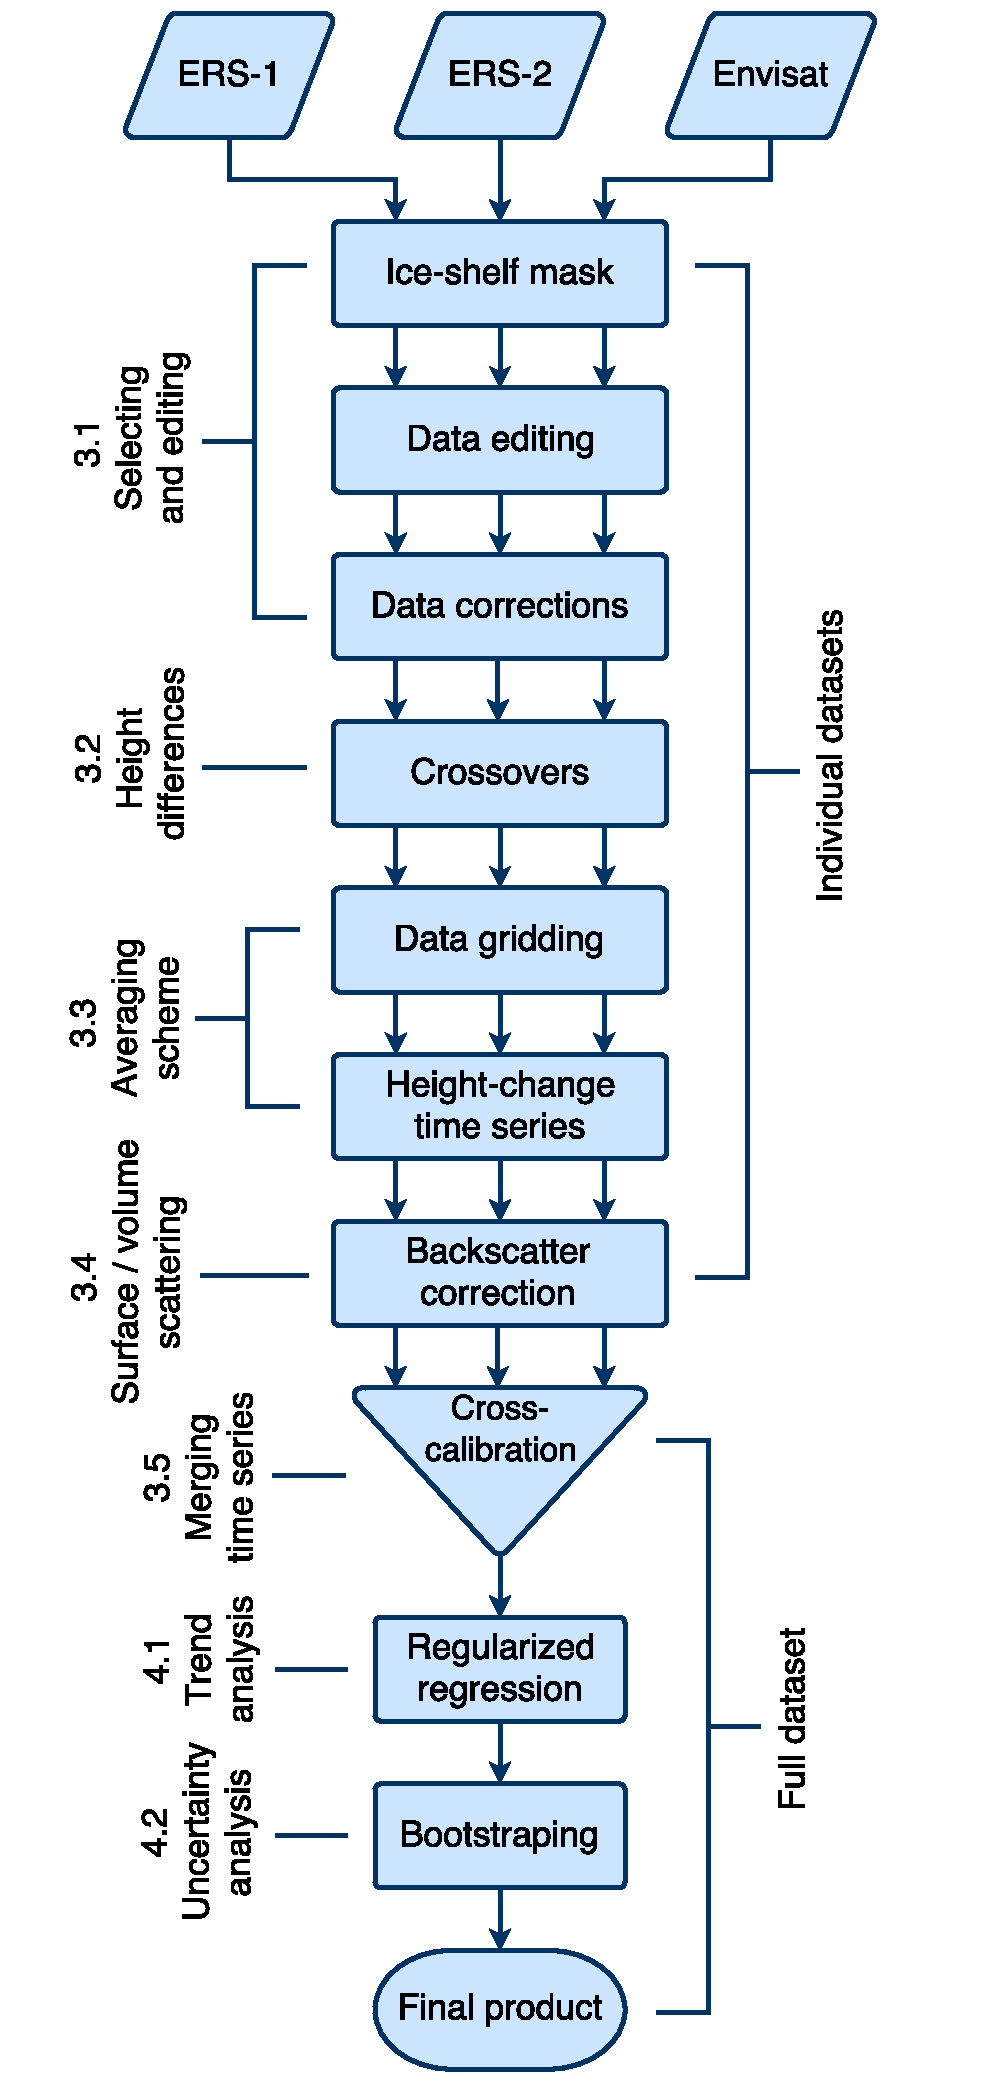
\includegraphics[width=\textwidth]{../img/flowchart_v4.pdf}
  \caption{Flowchart of our RA data processing scheme, showing the steps performed to construct an 18-year record of ice-shelf surface-height change from multiple satellite altimeters. Each step is described in Sections \ref{ra-processing} and \ref{ra-analysis}.}
  \label{c2f2}
\end{figure}

\subsubsection{Additional data corrections}

The ocean tide corrections applied to the IDR (from the CSR3 global tide model) are not accurate in Antarctica \parencite{King2005}; for that reason, we removed this correction from the data and applied an improved tide correction using the regional Circum-Antarctic Tidal Simulation model (CATS2008a), an updated version of the inverse tide model described by \parencite{Padman2002}. This tide model has higher resolution ($\sim$4 km) and a more accurate land mask than global models, resulting in more accurate tide prediction close to the coast. We also corrected for the ocean tidal loading (the elastic deformation of the seabed in response to the tide load) using the TPXO7.2 model \parencite{Egbert2002}.

\subsubsection{Estimating height differences}

To estimate the height differences at crossovers we first precisely locate the intersection points between each ascending and descending satellite track. We then find the two data points on either side of this intersection for each track pair, interpolate these to estimate the height at actual crossover location, and difference values from both tracks. When some data are missing along the satellite track, we only estimated crossover height-differences if the gap between data points on either side of the intersection point was less than 3 km. This criterion ensured that the RA pulse-limited footprints at both ends of the gap still overlapped sufficiently that interpolated heights along both tracks at the precise crossover location were consistent representations of the same location on the ice surface.

Our approach to developing time series of ice-shelf height with respect to an initial epoch $t_0$, $h(t-t_0)$, uses a multi-reference time scheme \parencite{Khvorostovsky2012, Li2006} applied to each satellite mission separately. This method computes crossover height differences for each pair of ascending and descending tracks, $\Delta h(t_i,t_j)$, throughout the entire record for a specific mission regardless of time separation between track pairs. For example, in the 9-year Envisat record, time separation of differences, $\Delta t=t_j-t_i$, at crossovers range from close to zero to nine years. 

For ERS-1, where data were acquired in different modes ('ice' and 'ocean') at different times over the ice shelves, we analyzed the crossovers $\Delta h(t_i,t_j)$ estimated from pairs of tracks with the same operation mode (ice-mode crossed with ice-mode or ocean-mode crossed with ocean-mode). Results for both modes were practically identical. In contrast, estimates of $\Delta h(t_i,t_j)$ obtained from a mixed-mode crossover (one track in ice-mode, the other in ocean-mode), were not consistent with the same-mode pairings. We also found that ice-mode data by itself was insufficient to provide near-full coverage over the ice shelves for the first few years of ERS-1 operation. Hence, for ERS-1 we retained both types of same-mode crossovers (ice-ice and ocean-ocean). For Envisat we used the fine-mode data only. 

\subsection{Averaging to enhance the signal-to-noise ratio}

For a given change in ice thickness, the estimated height-change signal over a floating ice shelf is about an order of magnitude smaller than the same signal over grounded ice. This is because, outside of a narrow ice-flexure zone roughly 1--10 km wide seaward of the grounding line, ice shelves are in hydrostatic equilibrium with a density that is about 10\% less than seawater. Since ice thickness and mass are the primary variables we wish to document, this reduced signal implies that there is a need to reduce the noise in the height estimates over ice shelves, a problem that is compounded when the goal is to identify variability over short time scales.

To enhance the signal-to-noise ratio over floating ice we implemented two averaging steps to reduce the variance in the height estimates, as described below.

\subsubsection{Spatial gridding and temporal binning}

We defined blocks of height data, $h(\mathbf{x},t_i)$, consisting of all ascending and descending tracks within non-overlapping 3-month time bins and spatial grid cells of 0.75$^\circ \times 0.25^\circ$ in longitude and latitude, respectively ($\sim30 \times 30$ km at 71$^\circ$S). At shorter time intervals, e.g., one month, the data records are often discontinuous. Aggregating data over 3-month bins provides continuous records while still resolving the annual cycle. The choice of grid-cell size ($\sim$30 km) was a compromise between characteristic spatial scales of ice-shelf processes and the spatial distribution of crossovers (Figure \ref{c2f1}). We identify each 3-dimensional block (one time bin and spatial cell), by its central time, $t_i \rightarrow i=0,1,2,..,N$, where $N$ is the total number of time bins within each satellite record, and by its central location, $\mathbf x \rightarrow 0^\circ <$ longitude $< 360^\circ$ and $-81.5^\circ <$ latitude $< -64.5^\circ$ (the center of the grid cells).

For each pair of blocks for the same cell but for separate time bins $t_i$ and $t_j$, we developed the set of all track-crossing-point height differences, ${\Delta h(t_i,t_j)}$, found by differencing all height values from the two data blocks. During this process we excluded crossover values higher than 15 m (gross outliers). For all pairs of ${t_i,t_j}$, we therefore obtained average height changes at each location as

\begin{equation}
  \overbar{\Delta h}(\mathbf{x}, t_i, t_j) = \frac{1}{n_\text{ad} + n_\text{da}} 
  \left\{
  n_\text{ad} \, \text{Md}\!\left[ \Delta h_\text{ad}(t_i, t_j) \right] +
  n_\text{da} \, \text{Md}\!\left[ \Delta h_\text{da}(t_i, t_j) \right]
  \right\}
  \label{c2e1}
\end{equation}

\noindent
where $\overbar{\Delta h}$ is the weighted-mean height-change estimate between times $t_i$ and $t_j$, $\Delta h_\text{ad}$ and $\Delta h_\text{da}$ are height changes formed by differencing ascending-descending and descending-ascending satellite ground tracks, respectively, $n_ad$ and $n_da$ are the number of crossovers of each type per block, and $\text{Md}[\,]$ is the median operator. We used the median instead of the mean because individual values of $\Delta h(t_i,t_j)$ can have large errors and its distribution can be non-Gaussian. It is necessary to use the average between ascending/descending and descending/ascending crossovers to remove any time-invariant biases, such as those introduced by the combination of satellite orientation, antenna polarization and ice surface anisotropy.

If we assume that true temporal variations in $h$ are small for small time separations (within the time bin itself, {\it i.e.}, less than three months), then the statistics of $\Delta h(t_i,t_j)$ are a measure of noise in the height difference estimates. This noise value may be spatially dependent; for example, relatively smooth and flat regions of ice shelf may have smaller noise in $\Delta h$ than regions where the ice-shelf surface is sloping or rough.

\subsubsection{Derivation of height-change time series}

The simplest way to obtain a time series of height change for a specific spatial cell is to difference the first block of data consecutively with all subsequent blocks \parencite[E.G.,]{Zwally1989}. This approach, however, results in all height differences in the resulting record being dependent upon the quality and data availability of the reference epoch (the first block). Instead, for each cell we evaluated all possible combinations between time bins within each satellite mission \parencite{Li2006}, and further combinations between the formed differences as in \textcite{Khvorostovsky2012}. This procedure was carried out as follows.

For each grid cell we constructed a set of $N-1$ time series of average height differences with respect to each of the $N-1$ separate epochs, and then formed a full matrix (one per cell) containing one height-change record per row. For example, taking $t_0$ to be the reference epoch (any time could be chosen) we then have:

\begin{equation}
  [\Delta h] = 
  \begin{pmatrix}
    h_{0,1} & h_{0,2} & h_{0,3} & \cdots & h_{0,N} \\
    -- & h_{0,1} + h_{1,2} & h_{0,1} + h_{1,3} & \cdots & h_{0,1} + h_{1,N} \\
    h_{0,2} - h_{1,2} & -- & h_{0,2} + h_{2,3} & \cdots & h_{0,2} + h_{2,N} \\
    h_{0,3} - h_{1,3} & h_{0,3} - h_{2,3} & -- & \cdots & h_{0,3} + h_{3,N} \\
    \cdots & \cdots & \cdots & \cdots & \cdots \\
    h_{0,N} - h_{1,N} & h_{0,N} - h_{2,N} & h_{0,N} - h_{3,N} & \cdots & --
  \end{pmatrix}
  \label{c2e2}
\end{equation}

\noindent
where $h_{i,j} = \overbar{\Delta h}(\mathbf{x}, t_i, t_j)$ from Eq. (\ref{c2e1}). In the example above, every row constitutes a time series of height change with respect to $t_0$. This is accomplished by (i) forming the upper triangle of the matrix from the calculated average differences, (ii) forming the lower triangle as the negative of the upper one, and (iii) using the elements of the first row (time series with respect to $t_0$) to reference each of the other rows (Figure \ref{c2f3}). We note that any row in the matrix could be used as the reference series ({\it i.e.}, any epoch); the optimal one, however, will cover the largest time span in the presence of data gaps.

Next, we weight-averaged the matrix rows by the number of crossovers used to form each average difference to produce a mean time series per cell, with reduced statistical error:

\begin{equation}
  h(\mathbf x, \tau) = \langle [\Delta h] \rangle 
  \label{c2e3}
\end{equation}

\noindent
where $\tau = t - t_0$. We propagated individual errors in the averaging procedure assuming normality \parencite{Li2006}.

To evaluate possible signal aliasing we used a small region to test aggregating data in 3-month bins that were overlapped by $1/3$ as in \textcite{Khvorostovsky2011}. The overlapping approach required a much longer computation time, and the resulting average time series were the same as the non-overlapping approach, and so we did not apply this to the full dataset.


\begin{figure}[!ht]
  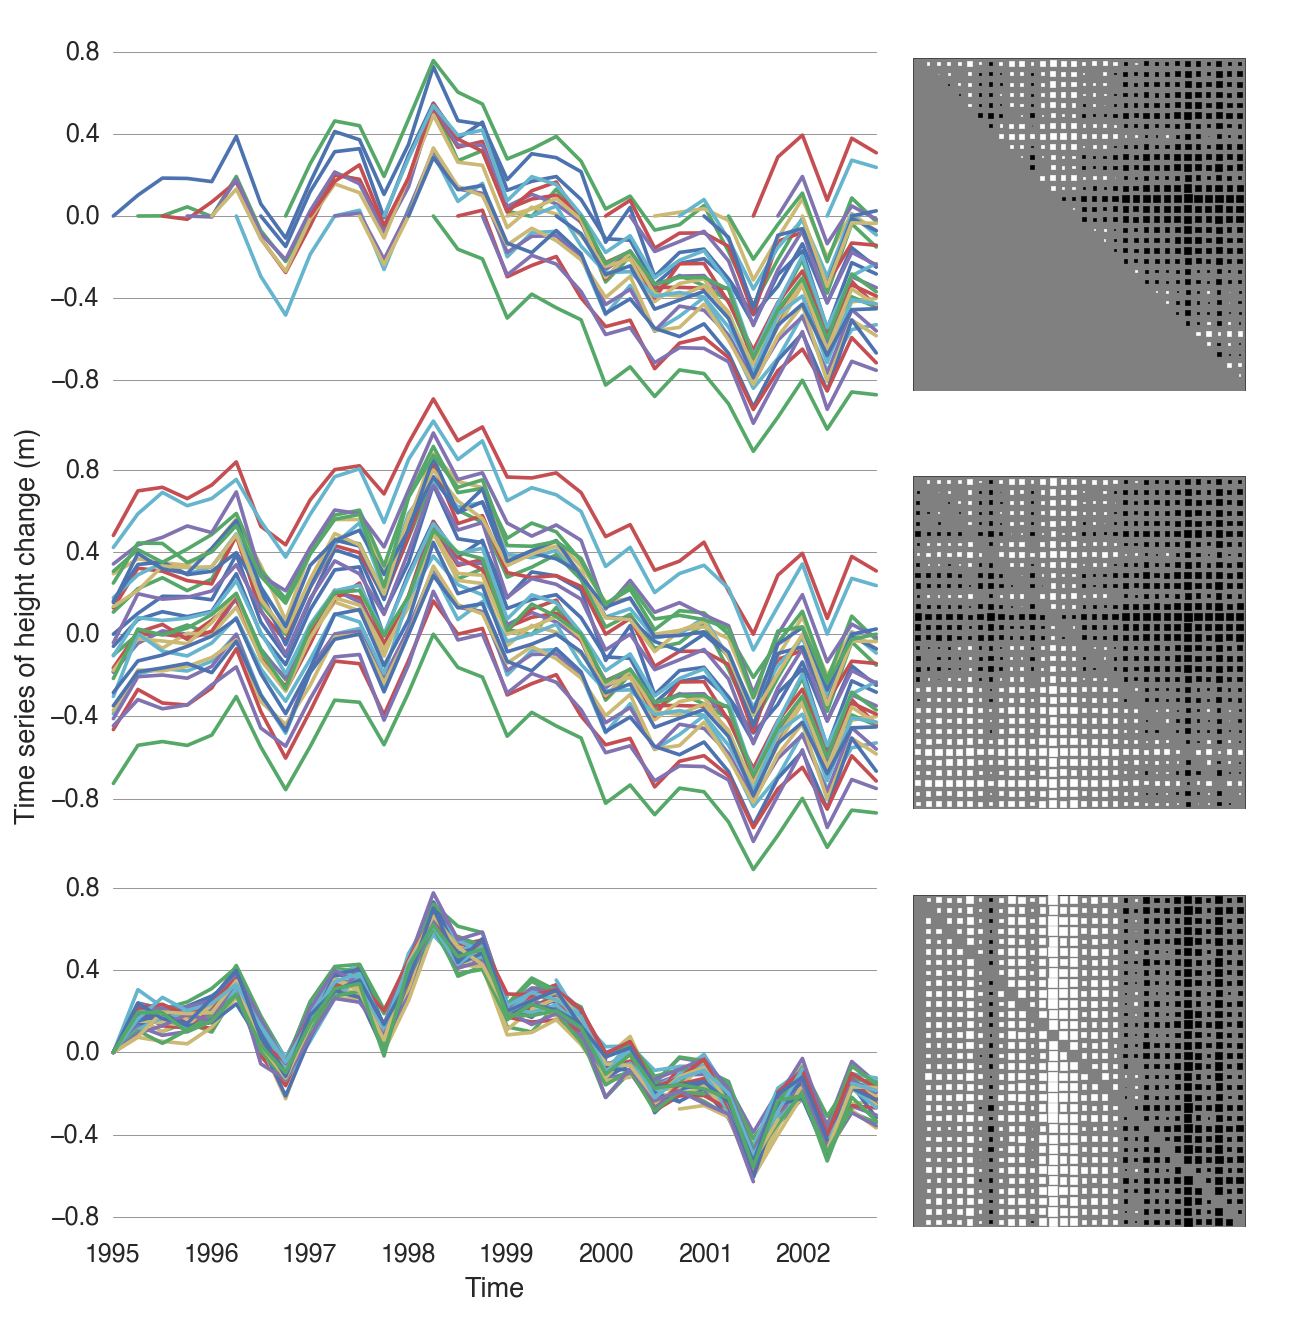
\includegraphics[width=\textwidth]{../img/multiref_matrix_v4.png}
  \caption{
  Representation of the multi-reference time series approach. (left) Individual time series of cumulative change. (right) Diagram representing the matrix formed with the time series on the left (one time series per row). From top to bottom is depicted the process of forming single-grid-cell average time series: (top) the one-sided matrix of average differences; (middle) the two-sided matrix; (bottom) referencing all the rows (time series) to a common epoch for posterior averaging (this matrix is Eq. \ref{c2e2}).} 
  \label{c2f3}
\end{figure}

\subsection{Surface and volume scattering variation}

Interpreting heights derived from RA data over snow-covered ice surfaces requires an understanding of the complex interaction of the radar wave with the snowpack and firn (compressed snow that has not yet formed into solid ice). Over ice sheets, part of the incident radar energy penetrates into the snowpack/firn \parencite{Ridley1988} by an amount that depends on the properties of the surface layers including temperature, density, grain-size and moisture content \parencite{Davis1993}, leading to volume scattering with reflections within sub-surface layers and ice lenses. Volume scattering increases the path length of the radiation and, therefore, its travel-time back to the satellite and the inferred height. The waveform shape in the presence of volume scattering is also different than if only surface scattering occurred. In some cases, most of the echo can be from a well-defined sub-surface horizon within the snowpack \parencite{Thomas2008}, leading to a surface-like waveform shape, but a height estimate that is still lower than the true surface.

The penetration depth (where the radar pulse decays by $1/e$ of its initial intensity) varies with density, grain-size, and water content of the snow/firn. Penetration depth can be several meters over the colder and dryer parts of the Antarctic plateau where grain sizes are smaller but is much lower (on the order of centimeters) over the warmer and wetter ice shelves where grain sizes are larger \parencite{Davis1996}. To demonstrate this we used the \parencite{Davis1993} surface/volume algorithm to estimate the extinction coefficient ($k_\text{e}$; which is inversely proportional to penetration depth) for the entire Antarctic area under the ERS-1 satellite's coverage, using ERS-1 altimeter level-1 ocean-mode waveforms (Phase C) (Figure \ref{c2f4}). In general, $k_\text{e}$ is on the order of 4--5 times higher over the ice shelves than elsewhere on the ice sheet. This means that the penetration bias is not as large over the ice shelves as it is over the ice sheet interior.

The return radar waveform used to estimate the surface height is the sum of surface echo (energy scattered by the surface) and volume echo (energy scattered within the snowpack). Perturbations in the return radar waveform occur by changes in the properties of the snowpack, which alters the effective backscatter layer, potentially leading to a biased surface-height estimate. Two competing effects (with opposite signs) play a significant role in altering the shape of the return waveform: i) penetration of the signal into the firn layer increases volume scattering (increasing the waveform’s leading-edge width); and ii) densification of the surface increases the air-snow dielectric contrast (decreasing the leading-edge width). We investigated corrections to minimize these effects as described in Section \ref{bs-corr} below.


\begin{figure}[!ht]
  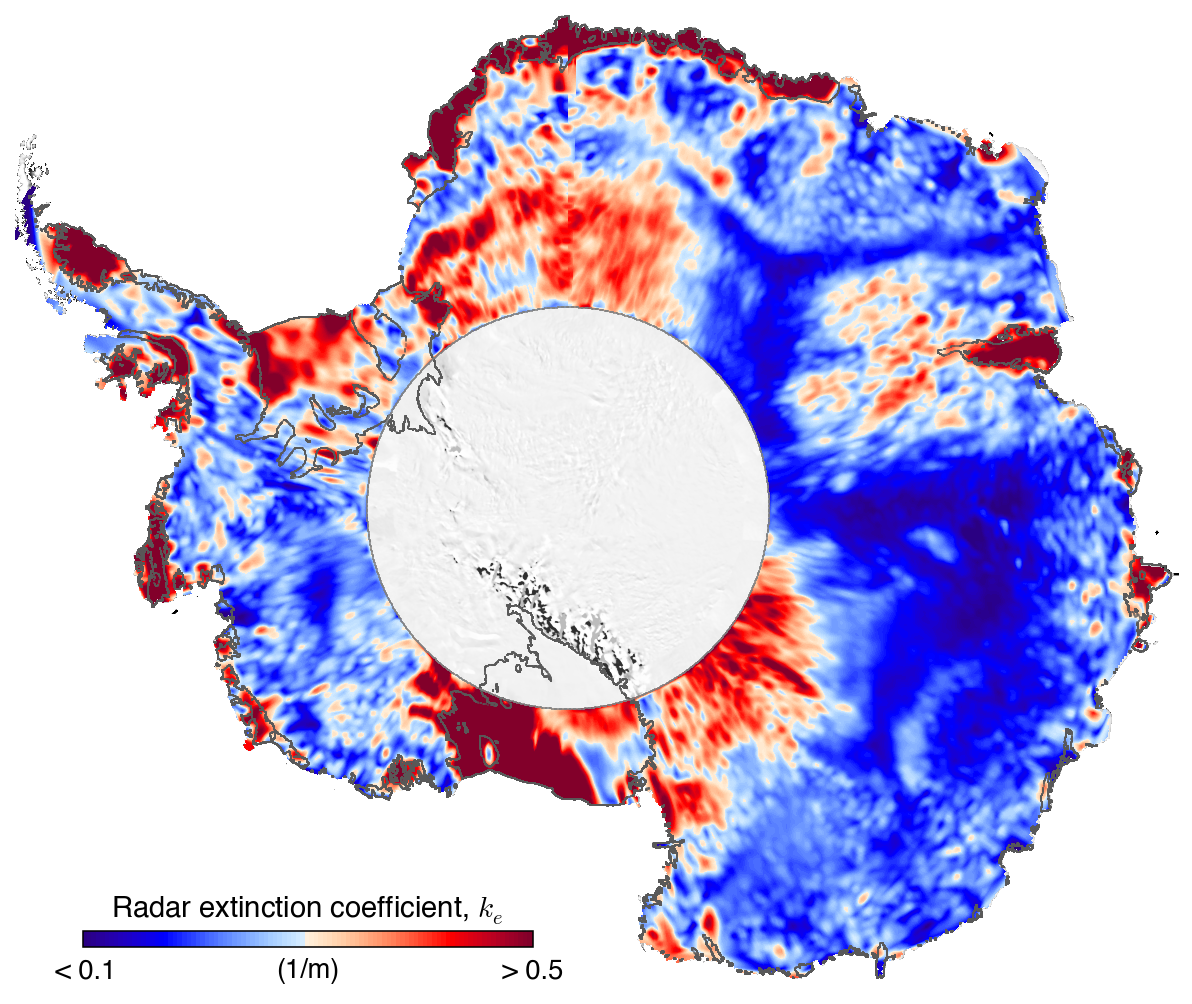
\includegraphics[width=\textwidth]{../img/extinction_coef_v3d.png}
  \caption{
  Estimated radar altimeter extinction coefficient ($k_\text{e}$) over the Antarctic ice sheet. $k_\text{e}$ was derived from ERS-1 Phase C ocean-mode return waveforms over the ice sheet and ice shelves using a surface/volume scattering algorithm \parencite{Davis1993}. Note that the $k_\text{e}$  (which is inversely related to the penetration depth) is generally higher in the ice shelves than on the plateau. This difference can mostly be explained in terms of grain sizes: on the ice shelf, individual particles are larger than those on the plateau, due to much warmer temperatures, combined with successive melt-freeze cycles ({\it i.e.}, wet snow metamorphosis) \parencite{Zwally1994}; therefore $k_\text{e}$ is high. On the plateau, grain sizes depend on surface temperature and accumulation rate. In general, as elevation and distance from the coast (continentally) increases, temperatures decrease; therefore the grain sizes and $k_\text{e}$ decrease.
  }
  \label{c2f4}
\end{figure}

\subsubsection{Correction for changes in backscatter}
\label{ra-corr}

Although much progress has been made in understanding the relation between backscatter fluctuation, resulting mainly from variations in near-surface properties, and altimeter-derived height \parencite{Arthern2001, Davis1993, Legresy1998, Partington1989, Remy2012, Ridley1988}, it is still an active area of investigation and its full impact on the RA measurement error remains poorly known \parencite{Remy2012}. To attempt to minimize the impact on the estimated height of fluctuations in backscatter, an empirical adjustment using backscatter information is performed \parencite{Davis2004, Khvorostovsky2012, Remy2009, Wingham2006, Wingham1998, Zwally2005}.

We used the altimeter automatic gain control (AGC) as a measure of backscattered power to adjust our height-change time series using corresponding series of changes in AGC, $g(\mathbf x,\tau)$. We formed these backscatter-change time series for each grid cell in the same way as the height-change series described above. We derived a spatially variant sensitivity factor, $S(\mathbf x)$, to scale the backscatter values at each grid-cell. This sensitivity is the regression slope of the correlation between height and backscatter changes that we derived independently for each RA mission. We then corrected each time series as follows:

\begin{equation}
  h(\mathbf x,\tau)_\text{cor} = h(\mathbf x,\tau) 
    - S(\mathbf x) \, g(\mathbf x,\tau) - h_0(\mathbf x)
  \label{c2e4}
\end{equation}

\noindent
where $h_\text{cor}$ is backscatter-corrected height-change, $S$ is the sensitivity factor (altimeter dependent), $g$ is gain change, and $h_0$ is the regression intercept (not needed for correcting full independent records relative to some epoch). For the regression procedure we used a robust method, M-estimator \parencite{Huber1981}, instead of the commonly used least-squares approach, which can be sensitive to outliers (especially when few data are available).

In selecting an optimal backscatter correction scheme we tested three different approaches. We correlated series of backscatter and height changes: i) using the cross-calibrated full 18-year records, ii) using data within 2 and 3-year sliding windows (similar to \textcite{Khvorostovsky2012}) and iii) using independent single-mission records. For each approach we performed the correlation using both the original time series (absolute values) and the differenced series (derivative). We found that the third approach was the only one to perform consistently under a variety of conditions ({\it e.g.}, high vs. low variance, high vs. low correlation, high vs. low heteroscedasticity). Note that using differenced series is equivalent to using high-pass filtered records and, therefore, higher correlations are expected since backscatter change is primarily a function of seasonality. However, in correlating differenced series only the short-term fluctuations in backscatter are being taken into account. Hence, we corrected our height-change records by correlating series of absolute values using (iii).

\subsubsection{Densification from changes in the firn column}

One approach to accounting for changing surface mass balance over an ice shelf, specifically firn compaction/densification, is to use an atmospheric-based model to predict how the firn column evolves under modeled climate conditions. For example, a laser altimeter study by \textcite{Pritchard2012} used modeling of changes in the firn column to isolate the part of the signal due to fluctuations in the snowpack. We performed a correlation analysis between our backscatter-uncorrected time series, which contain the seasonal response of the ice-shelf surface as detected by the altimeter's automatic gain control (backscatter), and the height changes derived from a firn densification model (FDM). To construct the firn height-change record we used the \textcite{Ligtenberg2011}’s FDM from which (i) we extracted firn height-change series for each location in our grid; (ii) averaged the 48-hour firn records with a 3-month moving window; and (iii) retained the discrete time-values that corresponded to our 3-month ice-shelf height records.

We found no correlation between the firn height changes and RA-derived changes in ice-shelf height at the fine resolution required for this study (individual grid cells of $\sim$30 km). The firn model was able to provide, however, an estimate of the expected seasonal variation of the firn height at the larger scale (Figure \ref{c2f5}). Additionally, since some degree of penetration through fresh snow is expected at the frequency of the Ku-band altimeter, satellite RAs are less sensitive than are laser altimeters to fluctuations in surface mass balance. For these reasons we found no justification to use a FDM to make any firn-change correction on RA height estimates.


\begin{figure}[!ht]
  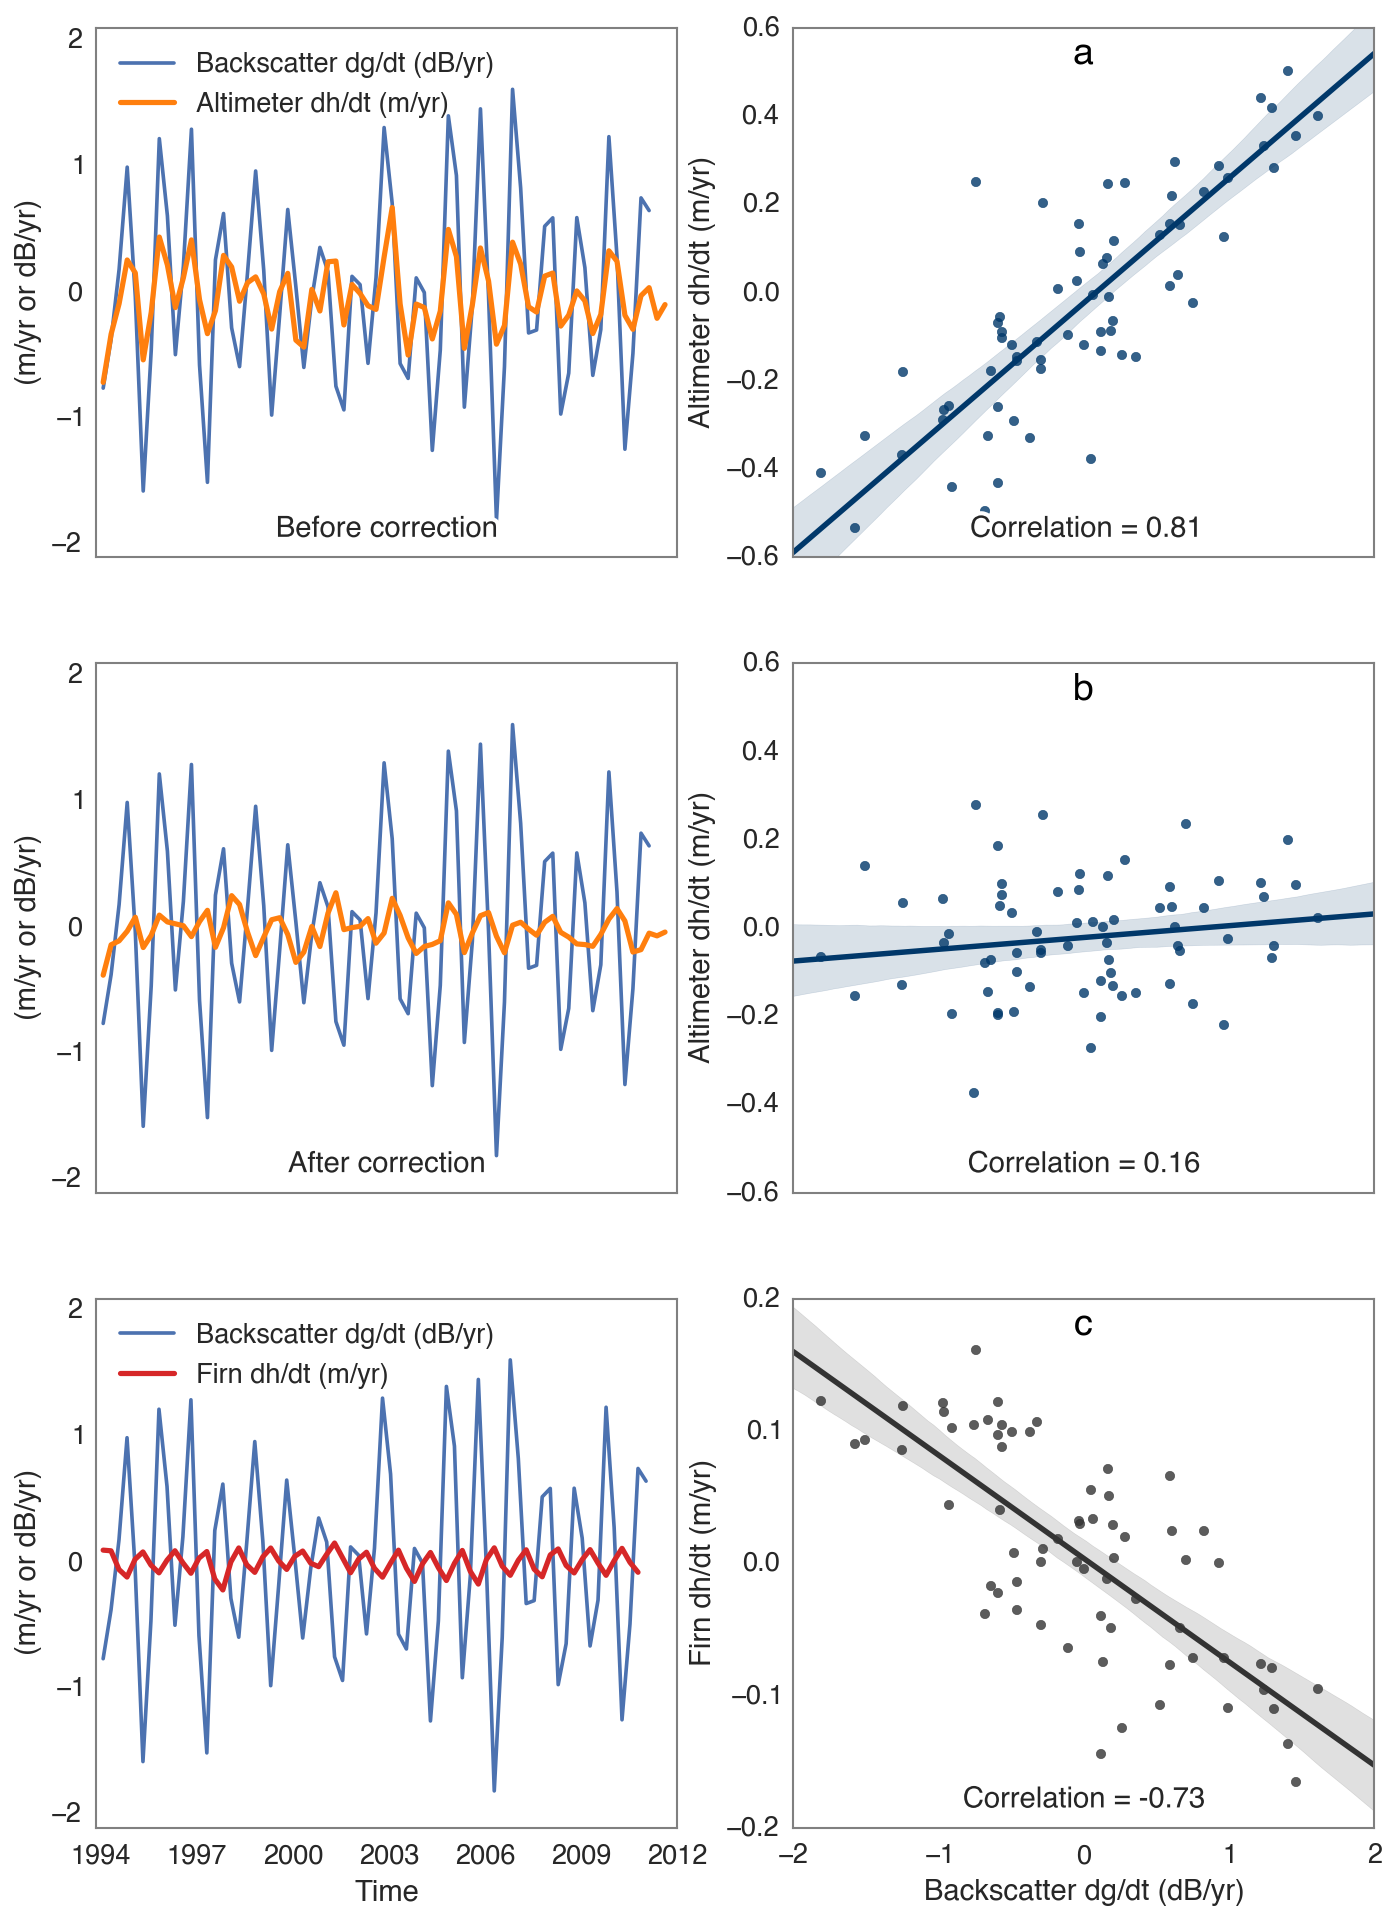
\includegraphics[width=\textwidth]{../img/correlation_h_b_f_v7.png}
  \caption{
  Correlation between backscatter (AGC), ice-shelf height and firn-height change derived from a firn densification model. (left column) Derivative of circum-Antarctic-wide average time series; (right column) respective correlations. From top to bottom, correlations between the derivative of backscatter and derivatives of: (a) uncorrected ice-shelf height; (b) corrected ice-shelf height (at the grid-cell level); and (c) firn-column height time series.
  } 
  \label{c2f5}
\end{figure}


